% -*- Mode:TeX -*-

%% IMPORTANT: The official thesis specifications are available at:
%%            http://libraries.mit.edu/archives/thesis-specs/
%%
%%            Please verify your thesis' formatting and copyright
%%            assignment before submission.  If you notice any
%%            discrepancies between these templates and the 
%%            MIT Libraries' specs, please let us know
%%            by e-mailing thesis@mit.edu

%% The documentclass options along with the pagestyle can be used to generate
%% a technical report, a draft copy, or a regular thesis.  You may need to
%% re-specify the pagestyle after you \include  cover.tex.  For more
%% information, see the first few lines of mitthesis.cls. 

%\documentclass[12pt,vi,twoside]{mitthesis}
%%
%%  If you want your thesis copyright to you instead of MIT, use the
%%  ``vi'' option, as above.
%%
%\documentclass[12pt,twoside,leftblank]{mitthesis}
%%
%% If you want blank pages before new chapters to be labelled ``This
%% Page Intentionally Left Blank'', use the ``leftblank'' option, as
%% above. 

\documentclass[11pt,twoside]{mitthesis}
\usepackage{lgrind}
%% These have been added at the request of the MIT Libraries, because
%% some PDF conversions mess up the ligatures.  -LB, 1/22/2014
\usepackage{cmap}
\usepackage[T1]{fontenc}
\usepackage{graphicx}
\usepackage{subfig}
\usepackage{xcolor}
\usepackage{amssymb}
\usepackage{algorithm}
\usepackage{algorithmicx}
\usepackage{algpseudocode}
\usepackage{bm}
\pagestyle{plain}



%% This bit allows you to either specify only the files which you wish to
%% process, or `all' to process all files which you \include.
%% Krishna Sethuraman (1990).

%\typein [\files]{Enter file names to process, (chap1,chap2 ...), or `all' to
%process all files:}
%\def\all{all}
%\ifx\files\all \typeout{Including all files.} \else \typeout{Including only \files.} \includeonly{\files} %\fi

\def\files{all}

\begin{document}

% -*-latex-*-
% 
% For questions, comments, concerns or complaints:
% thesis@mit.edu
% 
%
% $Log: cover.tex,v $
% Revision 1.8  2008/05/13 15:02:15  jdreed
% Degree month is June, not May.  Added note about prevdegrees.
% Arthur Smith's title updated
%
% Revision 1.7  2001/02/08 18:53:16  boojum
% changed some \newpages to \cleardoublepages
%
% Revision 1.6  1999/10/21 14:49:31  boojum
% changed comment referring to documentstyle
%
% Revision 1.5  1999/10/21 14:39:04  boojum
% *** empty log message ***
%
% Revision 1.4  1997/04/18  17:54:10  othomas
% added page numbers on abstract and cover, and made 1 abstract
% page the default rather than 2.  (anne hunter tells me this
% is the new institute standard.)
%
% Revision 1.4  1997/04/18  17:54:10  othomas
% added page numbers on abstract and cover, and made 1 abstract
% page the default rather than 2.  (anne hunter tells me this
% is the new institute standard.)
%
% Revision 1.3  93/05/17  17:06:29  starflt
% Added acknowledgements section (suggested by tompalka)
% 
% Revision 1.2  92/04/22  13:13:13  epeisach
% Fixes for 1991 course 6 requirements
% Phrase "and to grant others the right to do so" has been added to 
% permission clause
% Second copy of abstract is not counted as separate pages so numbering works
% out
% 
% Revision 1.1  92/04/22  13:08:20  epeisach

% NOTE:
% These templates make an effort to conform to the MIT Thesis specifications,
% however the specifications can change.  We recommend that you verify the
% layout of your title page with your thesis advisor and/or the MIT 
% Libraries before printing your final copy.
\title{A Hybrid Continuum and Discrete Element Method for Granular Media Modeling}

\author{Maytee Chantharayukhonthorn}
% If you wish to list your previous degrees on the cover page, use the 
% previous degrees command:
%       \prevdegrees{A.A., Harvard University (1985)}
% You can use the \\ command to list multiple previous degrees
%       \prevdegrees{B.S., University of California (1978) \\
%                    S.M., Massachusetts Institute of Technology (1981)}
\department{Department of Mechanical Engineering}

% If the thesis is for two degrees simultaneously, list them both
% separated by \and like this:
% \degree{Doctor of Philosophy \and Master of Science}
\degree{Master of Science in Mechanical Engineering}

% As of the 2007-08 academic year, valid degree months are September, 
% February, or June.  The default is June.
\degreemonth{June}
\degreeyear{2019}
\thesisdate{May 19, 2019}

%% By default, the thesis will be copyrighted to MIT.  If you need to copyright
%% the thesis to yourself, just specify the `vi' documentclass option.  If for
%% some reason you want to exactly specify the copyright notice text, you can
%% use the \copyrightnoticetext command.  
%\copyrightnoticetext{\copyright IBM, 1990.  Do not open till Xmas.}

% If there is more than one supervisor, use the \supervisor command
% once for each.
\supervisor{Kenneth Kamrin}{Associate Professor}

% This is the department committee chairman, not the thesis committee
% chairman.  You should replace this with your Department's Committee
% Chairman.
\chairman{Evelyn Wang}{Chairman, Department Committee on Graduate Theses}

% Make the titlepage based on the above information.  If you need
% something special and can't use the standard form, you can specify
% the exact text of the titlepage yourself.  Put it in a titlepage
% environment and leave blank lines where you want vertical space.
% The spaces will be adjusted to fill the entire page.  The dotted
% lines for the signatures are made with the \signature command.
\maketitle

% The abstractpage environment sets up everything on the page except
% the text itself.  The title and other header material are put at the
% top of the page, and the supervisors are listed at the bottom.  A
% new page is begun both before and after.  Of course, an abstract may
% be more than one page itself.  If you need more control over the
% format of the page, you can use the abstract environment, which puts
% the word "Abstract" at the beginning and single spaces its text.

%% You can either \input (*not* \include) your abstract file, or you can put
%% the text of the abstract directly between the \begin{abstractpage} and
%% \end{abstractpage} commands.

% First copy: start a new page, and save the page number.
\cleardoublepage
% Uncomment the next line if you do NOT want a page number on your
% abstract and acknowledgments pages.
% \pagestyle{empty}
\setcounter{savepage}{\thepage}
\begin{abstractpage}
% $Log: abstract.tex,v $
% Revision 1.1  93/05/14  14:56:25  starflt
% Initial revision
% 
% Revision 1.1  90/05/04  10:41:01  lwvanels
% Initial revision
% 
%
%% The text of your abstract and nothing else (other than comments) goes here.
%% It will be single-spaced and the rest of the text that is supposed to go on
%% the abstract page will be generated by the abstractpage environment.  This
%% file should be \input (not \include 'd) from cover.tex.
Capturing the propagation of microscale physics to macroscale phenomena is intractable for many large systems. Scale propagation is a major issue in granular media, wherein two extremes are often taken. In one, granular materials are modeled as a continuum, which greatly reduces the number of degrees of freedom that describe the system and can thus be simulated relatively quickly. However continuum models are not always precise and have difficulty capturing certain effects such as particle size dependence. In discrete element methods (DEM), every grain and the interactions between them are simulated. DEM is accurate but solve time scales poorly with large grain numbers. Here, we present a hybrid simulation scheme, which seeks a best-of-both-worlds solution by bridging these two approaches.

A mass of granular media is partitioned into three domains: a continuum domain represented using the material point method (MPM), discrete grains using DEM, and a transition zone of both MPM and DEM that are coupled via kinematic constraints. An “oracle” determines which areas of the domain are MPM and which are DEM, and converts between the two. In the canonical example of silo flow, flow with a sufficiently small orifice jams, resolving length scale dependent effects. Collapse of granular columns modeled with the hybrid method compare quantitatively well with pure discrete simulation and experiments in literature. A significant speedup is seen with the hybrid method over a similar domain of pure discrete grains.
\end{abstractpage}

% Additional copy: start a new page, and reset the page number.  This way,
% the second copy of the abstract is not counted as separate pages.
% Uncomment the next 6 lines if you need two copies of the abstract
% page.
% \setcounter{page}{\thesavepage}
% \begin{abstractpage}
% % $Log: abstract.tex,v $
% Revision 1.1  93/05/14  14:56:25  starflt
% Initial revision
% 
% Revision 1.1  90/05/04  10:41:01  lwvanels
% Initial revision
% 
%
%% The text of your abstract and nothing else (other than comments) goes here.
%% It will be single-spaced and the rest of the text that is supposed to go on
%% the abstract page will be generated by the abstractpage environment.  This
%% file should be \input (not \include 'd) from cover.tex.
Capturing the propagation of microscale physics to macroscale phenomena is intractable for many large systems. Scale propagation is a major issue in granular media, wherein two extremes are often taken. In one, granular materials are modeled as a continuum, which greatly reduces the number of degrees of freedom that describe the system and can thus be simulated relatively quickly. However continuum models are not always precise and have difficulty capturing certain effects such as particle size dependence. In discrete element methods (DEM), every grain and the interactions between them are simulated. DEM is accurate but solve time scales poorly with large grain numbers. Here, we present a hybrid simulation scheme, which seeks a best-of-both-worlds solution by bridging these two approaches.

A mass of granular media is partitioned into three domains: a continuum domain represented using the material point method (MPM), discrete grains using DEM, and a transition zone of both MPM and DEM that are coupled via kinematic constraints. An “oracle” determines which areas of the domain are MPM and which are DEM, and converts between the two. In the canonical example of silo flow, flow with a sufficiently small orifice jams, resolving length scale dependent effects. Collapse of granular columns modeled with the hybrid method compare quantitatively well with pure discrete simulation and experiments in literature. A significant speedup is seen with the hybrid method over a similar domain of pure discrete grains.
% \end{abstractpage}

\cleardoublepage

\section*{Acknowledgments}
First and foremost I thank my family, whose love and support have made my academic journey possible. My parents have sacrificed much for the opportunities afforded to me, and completing this work is only the smallest of payments towards that debt.

Secondly I thank everyone involved in my academic career. I reserve most thanks to Ken Kamrin, my advisor who has guided me these past three years. I have learned much under him and I know I will gain much more in the years forward. I express gratitude towards the members of the Kamrin group, whose company has been both academically enlightening and greatly entertaining throughout my time in that 1-314 office. I also have deep gratitude for my collaborators in the Grinspun group: Yonghao Yue, Breannan Smith, Peter Chen, and Eitan Grinspun himself for being both great people and great researchers.

And of course I thank all of my friends who have supported me throughout my time at MIT, though a special thanks goes to two people in particular. Ani Chiti has been the source of much great conversation and perspective, and whose own academic journey I derive inspiration from. And finally I thank Grace Liu, who has been my emotional rock for the past three years. Graduate school has been a time of great peaks but also the occasional deep valley, and I would have never been able to make it past those valleys without her love by my side.


%%%%%%%%%%%%%%%%%%%%%%%%%%%%%%%%%%%%%%%%%%%%%%%%%%%%%%%%%%%%%%%%%%%%%%
% -*-latex-*-

% Some departments (e.g. 5) require an additional signature page.  See
% signature.tex for more information and uncomment the following line if
% applicable.
% % -*- Mode:TeX -*-
%
% Some departments (e.g. Chemistry) require an additional cover page
% with signatures of the thesis committee.  Please check with your
% thesis advisor or other appropriate person to determine if such a 
% page is required for your thesis.  
%
% If you choose not to use the "titlepage" environment, a \newpage
% commands, and several \vspace{\fill} commands may be necessary to
% achieve the required spacing.  The \signature command is defined in
% the "mitthesis" class
%
% The following sample appears courtesy of Ben Kaduk <kaduk@mit.edu> and
% was used in his June 2012 doctoral thesis in Chemistry. 

\begin{titlepage}
\begin{large}
This doctoral thesis has been examined by a Committee of the Department
of Chemistry as follows:

\signature{Professor Jianshu Cao}{Chairman, Thesis Committee \\
   Professor of Chemistry}

\signature{Professor Troy Van Voorhis}{Thesis Supervisor \\
   Associate Professor of Chemistry}

\signature{Professor Robert W. Field}{Member, Thesis Committee \\
   Haslam and Dewey Professor of Chemistry}
\end{large}
\end{titlepage}


\pagestyle{plain}
  % -*- Mode:TeX -*-
%% This file simply contains the commands that actually generate the table of
%% contents and lists of figures and tables.  You can omit any or all of
%% these files by simply taking out the appropriate command.  For more
%% information on these files, see appendix C.3.3 of the LaTeX manual. 
\tableofcontents
\newpage
\listoffigures
\newpage
\listoftables


%% This is an example first chapter.  You should put chapter/appendix that you
%% write into a separate file, and add a line \include{yourfilename} to
%% main.tex, where `yourfilename.tex' is the name of the chapter/appendix file.
%% You can process specific files by typing their names in at the 
%% \files=
%% prompt when you run the file main.tex through LaTeX.
\chapter{Introduction}

Modeling is a game of balance. Tractability and reasonable solution times fight against the physical realities of vast length and time scales. The assumptions one makes when formulating a model directly impact the solution methods that can be brought to bear to the problem at hand. There are almost always guaranteed trade-offs between the level of simplification of a model and the amount of time needed to solve that model.

Granular media present an interesting intermediary between the world of the discrete and the continuum. While oftentimes they are studied in contexts where continuum approximations are appropriate (i.e. geological), their behavior at much smaller length scales (a bucket of sand at the beach or flow through an hour glass) are still of great interest. However at those more everyday scales, the length scale of a single grain of sand is a relatively large proportion of the scale of the entire problem, and thus cannot be ignored. And even at the larger aforementioned geological scales, the initiation of an earthquake, for an example, still relies on individual grains of sand slipping and deforming against each other.

The great challenge, then is to formulate a model that can capture length scale effects but still have enough simplifying assumptions to make the problem solvable with efficient methods. This however seems to fly in the face of the modeling trade-off previously discussed; it is nearly impossible to have a single model that allows for fine-scale resolution and yet ignores those small length scales to become efficiently solvable. The solution we now propose addresses this issue by ignoring the "single" part of the "single model" clause, and instead hybridizes two distinct models to yield the two distinct attributes desired: resolution of length scale while maintaining efficient solvability. It is noted that the current work focuses on cohesionless granular systems, and thus approximate dry granular systems with no sources of attraction, like liquid bridges or electrostatic charges. This work is an elaboration and expansion of the work shown in Yue et al \cite{HG:2018}.

The work is structured as follows. The remainder of chapter 1 puts the current work in the greater academic context and discusses prior work on the modeling of granular media. Hybridization models in and out of granular media contexts are also discussed. 

Chapter 2 discusses the discrete element method used and some details of its algorithmic solution. While the level of detail presented may seem overly exhaustive, it provides important context for where the hybridization technique interfaces with the discrete element method.

Chapter 3 discusses the continuum models used. The method used to solve these models, the Material Point Method, is also discussed in detail.

Chapter 4 introduces the hybridization technique. Its goal, formulation, and solution are discussed.

Chapter 5 shows examples of the hybridization technique at work, with comparisons to the discrete and continuum model solutions, as well as to literature.

Chapter 6 builds off of the work shown in the previous sections, and introduces new enrichment schemes that are needed for problems beyond the ones discussed in Chapter 5.

Finally chapter 7 concludes the thesis and discusses future work. 

\section{Granular Media Modeling}

The ubiquity of granular media in everyday life cannot be understated. We walk on it on trails, drive over it on roads \cite{sullivan06}, ingest it in our pharmaceuticals, and eat it in our meals. Slightly less directly, granular media is second only to water for the type of material most commonly handled in industry \cite{Richard:2005:Slow}. Granular materials also appear often in the context of special effects in visual media. CGI scenes at a beach or desert require realistic simulation of granular media, and the most straightforward way to do this is to solve physically realistic models for granular behavior. Despite this ubiquity, a comprehensive model that can capture the behavior of granular media remains elusive. 

\begin{figure}[htp] 
    \centering
        \includegraphics[width=0.4\textwidth]{figs/grain_bouncing.pdf}
    \caption{Bottom of an hourglass displaying three distinct granular phases.}
    \label{hourglass}
\end{figure}

While much of the difficulty stems from the length and time scale problems mentioned before, granular media is also unique from many other materials in its ability to transition between different states. This is clearly evident in a flowing hourglass, as shown in Figure \ref{hourglass}. At the bottom of the hourglass, settled sand acts as a solid, able to support compressive stress without flowing. At the top of the static pile is a region of grains flowing over the static region, acting like a liquid. In between the top and bottom of the hourglass the grains flow much like a dilute gas, with no cohesive structure and interacting via collisions.

Different models and solution techniques are able to capture granular behavior in a given state, though of course with trade-offs in accurately capturing behavior in other states. A summary of different methods are discussed. 

\subsection{Discrete Methods}
Perhaps the most straightforward way one could model a system of granular material is to model the grains themselves. Methods that model individual grains and the interactions between them fall under the umbrella of discrete methods. While this can be expensive for very large systems (greater than approximately 50,000 particles per core given current CPU capabilities), the one-to-one correspondence of a single simulated grain to a physical grain can produce accurate results. Discrete element methods can largely be broken down into two classes: penalty based methods and contact dynamics.

Penalty methods, as their names suggest, penalize the overlap of particles with some type of force that is a function of that overlap. The discrete element method (note that in some literature the term "discrete element method" is used to denote the larger class of what is here termed "discrete methods"), first formulated by Cundall and Strack, still enjoys much use due to its simplicity and accuracy \cite{Cundall:1979}. Even within the confines of the simplicity of the proposed method though, great generalizability can be realized by having a free choice of the penalty function. The advantages of course come at some cost. For example, a major drawback is that, depending on the choice of penalty function, multiple material parameters may need to be fit to experiment. The material parameters themselves may then put constraints on the computational solve time. To concretely demonstrate this point, many penalty models have some notion of an elastic parameter that must be tuned. However, most individual grains of sand are fairly stiff, with Young's moduli on the order of $100 GPa$ and densities on the order of $2000 kg/m^3$ \cite{Wang:2010}. These properties, combined with the small size of many grains (~0.1 mm in diameter), result in a large wave speed through the material that travels a small distance, and this must be resolved within a given time step. Implicit methods of course exist to alleviate this issue somewhat, but those come with the usual drawbacks of additional computational overhead elsewhere.

Contact dynamics on the other hand treats grains as completely rigid and allow no overlaps. They are then formulated as optimization problems, and more specifically, mixed linear complementarity formulations, minimizing some potential with a no overlap constraint. While the question of material properties is then largely avoided in these methods, the introduction of friction and other properties is much less straightforward than in the formulation of discrete element methods. The lack of material properties is also a double-edged sword of sorts, as while infinitely stiff grains are often a better approximation of a system of grains than computational grains that are extremely soft, the reality is that grains do have a finite, though large, stiffness. Capturing that finite stiffness and its consequences, such as a finite wave speed and non-negligible grain deformation, can be crucial in some applications. These properties are in fact important for the hybrid scheme, and will be discussed later.

A key characteristic of both classes of discrete methods is that they can easily capture all phases of discrete matter. If compressed by exterior forces or boundaries, they act like a solid, able to support load through the creation of force chains, much like physical granular media. The removal of these forces and boundaries, and/or the introduction of shear forces, causes grains to flow over other grains in a liquid-like fashion. Pouring a system of discrete grains will see the grains separate, capturing a granular gas.

Another property of discrete element methods is that they are able to elucidate particle level properties and dynamics that are difficult to gather from experiment. Photoelastic disks can be used to investigate force chains, such as in the pioneering work of Behringer et al and continued by the likes of Daniels et al \cite{Daniels:2017,Howell:1999}. However these photoelastic disks are made of relatively soft polymers and are mostly used to investigate 2D arrangements of disks, and not 3D arrangements of spheres. On the other hand, discrete element methods calculate inter-particle forces out of necessity and can thus report quantitative data for these contacts. Expanding from 2D to 3D is also a straightforward process, and every contact in a 3D system can be easily obtained. The dynamics of every single grain in a system modeled with discrete methods can also be tracked and studied, which can be done in experiment, but only with much difficulty and cost, i.e. methods such as X-ray tomography and CT scans \cite{Kim:2013}. While computational expenses can limit the size of simulated systems, physical limitations of scanning equipment can limit the size of an experimental system that can be studied, greatly hampering one of the key advantages of experiments over simulations in granular media: scale. 

Thus despite the drawbacks of discrete element methods, they are still popular and widely used in congruence with, and sometimes in the place of, physical experiment. The ability to accurately capture grain-scale level dynamics, and to obtain quantitative data for every grain and contact, means that they can effectively be treated as computational "ground truth" for simulated granular systems. When accuracy in a simulation is needed, discrete element methods can be used with confidence, at least compared to other methods.

\subsection{Continuum Models}
\begin{figure}[htp] 
    \centering
    \includegraphics[width=0.4\textwidth]{figs/Laconchita1995landslide.jpg}
    \caption{Aftermath of a landslide in La Conchita, California \cite{Laconchita}.}
    \label{landslide}
\end{figure}

As stated before, for large %(what constitutes "large" varies from system to system, though ~20 grain diameters per continuum element dimension is used as a rule of thumb granular systems),
systems one can ignore the fact that there are individual grains of sand, treat the system as a continuous granular medium, and retain many physical properties of the system. A classic example of this can be seen in Figure \ref{landslide}, which shows the aftermath of a landslide. A useful feature of the shown landslide is that a road can be seen that cuts through the hill, and acts as a deformation marker. The deformed shape is reminiscent of Poiseuille flow, suggesting that the moving bulk is well represented by a continuum.

The basis of continuum theory applied to granular media in fact goes back more than 200 years, with the pioneering work of Coulomb who proposed a relation between shear stress, pressure, and a coefficient of friction in a granular continuua, very similar in form to Coulomb friction \cite{Coulomb}. Since that initial proposal, granular continuum theory has been greatly expanded upon. The incorporation of additional complexity displayed in physical granular systems into the continuum theory have resulted in models that capture behavior such as critical-state, and anisotropy \cite{Schofield:1968:Critical}\cite{Dafalias:2004:Sand}.

Much work on granular continuum theory has been conducted in the fields of civil engineering and soil mechanics, where understanding the behavior of granular systems under load is crucial \cite{Roscoe:1958}. There is thus a large body of work on granular media in a solid phase, and continuum modeling of grains in this state is well understood. Granular gases too have been well investigated, with kinetic theory being effectively used to understand granular systems in this state.

The "liquid" flowing phase of granular materials has been much more difficult to model. It was only recently that a seminal study conducted by GDR MiDi suggested a possible model for flowing granular systems \cite{Midi:2004:Dense}. The rheological model posited, commonly referred to as the $\mu(I)$ relation ($\mu$ of I), suggests a yield condition similar to that suggested by Coulomb nearly half a century ago, but with a friction coefficient dependent on a nondimensional inertial number, $I$, which describes the ratio of inertia to confining pressures in a granular system. Further work by Jop and De Cruz provided empirical relations between the friction coefficient $mu$ and $I$ \cite{Jop:2006:Constitutive,Cruz:2008}. Further extensions of this model have since been proposed, and work continues to this day on clarifying the high and low inertia number bounds of the $mu(I)$ relation. 

All of the previously described models, while increasingly complex, still retain some simplicity in the sense that they are all local models. No length-scale is introduced, and thus no non-local effects are captured. This deficiency has been recently addressed by the work of Kamrin et al, who have proposed a non-local continuum model and thus introduce a notion of a length scale back into the continuum model \cite{Kamrin:2012:Nonlocal}. At first glance this seems provides a possible solution to the beginning stated problem of capturing length-scale effects while retaining the ability of efficient continuum equation solving methods. However, much additional work must be done to completely characterize these non-local models, and thus for now cannot be relied upon to have the fidelity of discrete methods which capture length-scale effects by their very nature.

\subsection{Related Hybridization Work}
The hybridization of two different methods that are suited to two different length scales is an idea that has been explored before in other contexts. Specifically, in crystal plasticity, molecular dynamics simulations have been hybridized with continuum models to better inform the continuum models of the finer-scale kinematics occuring at slip planes \cite{Tadmor:1996,Smith:2001,Shimokawa:2007,Zhang:2005,Dhia:1998}. In granular media, discrete methods have been coupled with finite element methods, but in a manner that differs from what we propose here. In such methods, the output of discrete element simulations are used at the quadrature points of a finite element method to construct strain and stress fields; the classic finite element method is then used to advect the continuum mesh. Arlequin-type methods are used to decompose overlapped discrete and continuum domains, which we follow in this study. The validity of these types of methods has only recently been explored \cite{Yan:2010}, with some work being done on analyzing when continuum methods and discrete methods are both accurate \cite{Rycroft:2009,Kamrin:2010,Kamrin:2014}. The potential practical use of these types of methods is explored, for example, in a study by Wellmann that used discrete methods to enrich the stress field around drill tips \cite{Wellmann:2012}.

A major goal of the current technique is to speed up simulations while maintaining some measure of accuracy in zones that do not need to be well resolved. Techniques exist that aim to simply speed up discrete method simulations while ignoring the resolution of stresses and strains in zones that do not need to be simulated well; however, these techniques are useful in that they provide ideas on how to decompose the simulation into regions that need to be well resolved and those that do not. The graphics community in particular are interested in these techniques, as what occurs out of view of the audience does not need to be resolved. For example, in zones of granular media that are deemed sufficiently stationary, grains are frozen and are not used in the update of subsequent time steps \cite{Smith:2005}. These techniques are well suited to flows such as rotating drums and collapsing sand piles or growing sand piles, where the core of those geometries remain steady over time \cite{McCarthy:1998,Hsu:2010,Zhu:2010,Bouchaud:1994}. We aim to build upon the ideas used in these at times disparate fields to formulate a physically and mechanically consistent decomposition of a simulation into discrete and continuum regimes.

%% This is an example first chapter.  You should put chapter/appendix that you
%% write into a separate file, and add a line \include{yourfilename} to
%% main.tex, where `yourfilename.tex' is the name of the chapter/appendix file.
%% You can process specific files by typing their names in at the 
%% \files=
%% prompt when you run the file main.tex through LaTeX.
\chapter{Discrete Element Method}
As described generally in Chapter 1, the discrete element method (DEM) models a system of grains by modeling each grain as a separate entity and calculates the dynamics of each grain by integrating what essentially amounts to $\Sigma\bold{f}=m\bold{a}$ through time. In 2D, each grain is modeled as a disk with a radius $r$, parameterized by three degrees of freedom: two for the center of mass position of the disk (held by a position vector $\bold{x_d}\subset\mathbb{R}^2$), and a third for the rotation of the disk relative to some rest state. The dynamics are captured by another three parameters: two for the center of mass velocity and a third for the angular velocity about the center of mass. In 3D this representation is generalized to a sphere, again with radius $r$ and six degrees of freedom: three for the center of mass ($\bold{x_d}\subset\mathbb{R}^3$) position and three for the angles that describe grain orientation. The dynamics analogously generalize to six parameters, with three for center of mass velocity and three for angular velocities. For a system of $K$ particles, the degrees of freedom of all particles can be concatenated into a single degree of freedom list, the generalized coordinate vector $\bold{q_d}$. In 2D, $\bold{q_d}\subset\mathbb{R}^{3K}$ and in 3D, $\bold{q_d}\subset\mathbb{R}^{6K}$. A generalized velocity vector, $v_d$ can be similarly defined, with $\bold{v_d}\subset\mathbb{R}^{3K}$ in 2D and $ \bold{v_d}\subset\mathbb{R}^{6K}$ in 3D. Momentum balance for the whole granular system can then be summarized with
$$M_d\bold{a_d}=\bold{f_d}(\bold{q_d},\bold{v_d},t)$$
where $M_d\subset\mathbb{R}^{3Kx3K}$ (2D) and $M_d\subset\mathbb{R}^{6Kx6K}$ (3D) is the mass matrix, $\bold{a_d}\subset\mathbb{R}^{3K}$ (2D) and $\bold{a_d}\subset\mathbb{R}^{6K}$ (3D) is the generalized acceleration vector, and $\bold{f_d}$ is the force vector that encapsulates all internal and external forces of the system. The evolution of the system configuration can then be described with 
$$\bold{\dot{q_d}}=\hat{\dot{\bold{q_d}}}(\bold{q_d},\bold{v_d},\bold{a_d})$$
where $\hat{\dot{\bold{q_d}}}$ is a function that encapsulates configuration updates.

\subsection{DEM Model} \label{DEM_Model}
The construction of $\bold{f_d}$, and specifically the contact model that goes into $\bold{f_d}$, has been the source of much work. Popular contact models include Hertzian contact and linear spring-dashpot systems, the latter of which we use \textcolor{red}{FINDREFERENCE}. While Hertzian contact in theory accounts for a nonlinear penalty force with respect to penetration depth due to geometric considerations not present in the simple Hookean spring model, the simplicity of the Hookean spring model along with its acceptable accuracy from literature motivate the latter's use in the current study \textcolor{red}{FINDREFERENCE}. 

\begin{figure}[htp] 
    \centering
    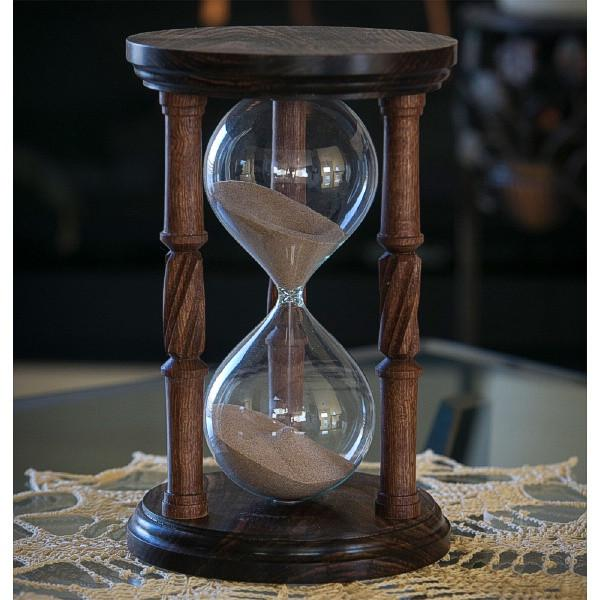
\includegraphics[width=0.4\textwidth]{figs/hourglass_whole.jpg}
    \caption{Two disks in contact with relevant properties labeled for DEM.}
    \label{DEM_diagram}
\end{figure}

In the current work, the contact force, $\bold{f_c}$, is a linear combination of a normal contact force $\bold{f_n}$ and tangential contact force $\bold{f_t}$, such that simply $\bold{f_c} = \bold{f_n} + \mu\bold{f_t}$, where $\mu$ is the coefficient of friction. $\bold{f_d}$ more concretely is
$$\bold{f_n}=k_nd\bold{n}-\gamma_n\bold{v_n}$$
where $k_n$ is the Hookean spring constant in the normal direction, $d$ is the penetration depth between the two disks, $\bold{n}$ is the contact normal unit vector, $\gamma_n$ is the normal damping coefficient, and $\bold{v_n}$ is the normal component of the relative velocity between the two disks. Similarly, the tangential contact force is given by
$$\bold{f_nt}=k_t\Delta\bold{s}-\gamma_t\bold{v_t}$$
where $k_t$ is the spring constant in the tangential direction, $\gamma_t$ is the tangential damping coefficient, and $\bold{v_t}$ is the tangential component of the relative velocity. Friction is captured in this model by requiring that
$$\bold{f_t}\leq\mu\bold{f_n}$$
which is accomplished by adjusting $\Delta\bold{s}$. For a given enduring contact over time, $\Delta\bold{s}$ for that contact is the time integral of the tangential relative velocity during that contact. $\Delta\bold{s}$ is then rescaled so that it $\bold{f_t}$ falls within the friction cone determined by $\mu\bold{f_n}$.

With the given spring-dashpot system, a coefficient of restitution (COR) $e$ can be tuned as a function of the model parameters. Given a desired $e$ and a normal spring coefficient $k_n$, $\gamma_n$ is determined as
$$\gamma_n=\sqrt{mk_n}(-2\log{e})/\sqrt{2(\pi^2+\log{e}^2}$$
where $m$ is the mean mass of a grain \cite{Kamrin:2014}. Note that the use of a "mean" mass is due to the fact that in all of the simulations conducted in this study, a slight polydispersity in granular radii is used with a single density for all particles, resulting in a mass distribution. This is done to better match real shape distributions in a granular system, and to avoid crystallization that commonly arises in monodisperse systems. The choice of $k_n$ and other material parameters is further explained for specific simulations later in the study, but in general is chosen to be as stiff as possible while still retaining a reasonable cost per time step, with a timestep usually on the order of $10^{-6}$ seconds.

\subsection{DEM Algorithm}
The DEM code used in this study was built completely in house, though is similar in general algorithmic structure to many DEM codes that exist, such as LAMMPS or LIGHTS \textcolor{red}{FINDREFERENCE}. Thus for transparency as well as necessity when later explaining the hybrid algorithm, the structure of the used DEM code is discussed.

\begin{algorithm}
  \caption{${\tt Overall \_ DEM \_ Algorithm}$}
  \begin{algorithmic}[1]
  \State ${\tt Broad\_Phase\_Collision\_Detection}$
  \For{$i=0 \dots num\_possible\_collisions$}
    \State ${\tt Narrow\_Phase\_Collision\_Detection}$
  \EndFor
  \State ${\tt Collision\_Update}$
  \For{$each\_collision\_type$}
    \State ${\tt Update\_Properties}$
    \State ${\tt Integrate\_\Delta\bold{s}}$
  \EndFor
  \State ${\tt Force\_Update}$ 
  \For{$each\_collision$}
    \State ${\tt Calculate\_Penalty\_Force}$
    \State ${\tt Correct\_\Delta\bold{s}}$
    \State ${\tt Add\_Force\_To\_Contact\_Grains}$
  \EndFor
  \State ${\tt Time\_Integration}$ 
  \end{algorithmic}
  \label{alg:DEM_algorithm}
\end{algorithm}

The $Broad\_Phase\_Collision\_Detection$ creates an axis-aligned bounding box (AABB) around each grain, and checks the intersection of those AABBs with a background grid. Each grid cell then has a vector of AABBs that intersect it, with each combination of AABB in that vector constituting a possible collision. All possible collisions are then looped over for an actual collision detection ($Narrow\_Phase\_Collision\_Detection$) and any real collisions are added to a vector of actual collisions for a given type. Collision types include, for example, circle\_circle collisions for grains in contact, or circle\_plane collisions for grains in contact with a rigid plane. The list of all collisions for every collision type are then looped over, and properties such as penetration depth and $\Delta\bold{s}$ are updated. With this information, a penalty force is calculated at every contact according to the model presented in \ref{DEM_Model}. With these forces, an explict Forward Euler update is used to numerically integrate the velocity of the grains, which is then used to integrate the position of the grains.

Though dry, cohesionless grains are the focus of the current work, it is noted that the DEM framework allows for a simple extension for cohesive grains. A new collison type can be defined that allows for tracking of grain interactions at a distance. As will be explained later, some initial work has in fact been done on this, by tracking liquid bridges that provide a source of cohesion in the system, in order to extend the hybrid method for cohesive systems.

As a final note, the DEM code is an extension and modification of the SCISIM code developed by Smith for contact dynamics \textcolor{red}{FINDREFERENCE}. In fact, as will be later discussed, that contact dynamics code was first used as the discrete method of choice for the hybrid project. However, the explicit penalty method was determined to better suit the needs of hybridization.
%% This is an example first chapter.  You should put chapter/appendix that you
%% write into a separate file, and add a line \include{yourfilename} to
%% main.tex, where `yourfilename.tex' is the name of the chapter/appendix file.
%% You can process specific files by typing their names in at the 
%% \files=
%% prompt when you run the file main.tex through LaTeX.
\chapter{Continuum Model}

\section{Hyperleastic-Plastic Model}

\section{Hypoelastic-Plastic Model}
In general, hypoelastic models differ from hyperelastic models in that the stress is not obtained from a gradient of a strain energy density function with respect to deformation. The specific hypoelastic granular continuum model used in this study was developed by Dunatunga and Kamrin \cite{Dunatunga:2015:Continuum}. To start one again begins with momentum balance and mass balance
$$\rho\frac{D\bold{v}}{Dt} = \nabla\cdot\bm{\sigma} + \rho\bold{b}$$
$$\frac{D\rho}{Dt} + \rho\nabla\cdot\bold{v}=0$$
with all terms similarly defined as in the hyperelastic model. A useful quantity, the spatial velocity gradient $\bold{L}$, is defined as
$$\bold{L}=\nabla\bold{v}$$
$\bold{L}$ can be decomposed into a symmetric part (known as the strain rate tensor) and skew part (known as the spin tensor), $\bold{D}$ and $\bold{W}$ respectively, such that
$$\bold{L}=\bold{D}+\bold{W}$$
$$\bold{D}=\frac{1}{2}(\bold{L}-\bold{L}^T)$$
$$\bold{W}=\frac{1}{2}(\bold{L}+\bold{L}^T)$$
In contrast to the hyperelastic model, the used hypoelastic model takes an additive split of the strain and strain rate-like terms into an elastic and plastic part. For example,
$$\bold{L}=\bold{L}^e+\bold{L}^p$$
The elastic and plastic spatial velocity gradients can then be decomposed into spin and strain rate tensors
$$\bold{L}^e=\bold{D}^e+\bold{W}^e$$
$$\bold{L}^p=\bold{D}^p+\bold{W}^p$$
A commonly taken assumption that is also taken here is one of spin-less plastic flow, so that $\bold{W}^p=\bold{0}$ and $\bold{L}^p=\bold{D}^p$. Plastic flow codirectionality with the stress deviator and isochoric plastic flow are also taken as assumptions, leading to an plastic flow rate of
$$\bold{L}^p=\bold{\hat{D}}^p(\bm{\sigma})=\frac{1}{\sqrt{2}}\dot{\bar{\gamma}}^p(\bm{\sigma})\frac{\bm{\sigma}_0}{||\bm{\sigma}_0||}$$
where $\dot{\bar{\gamma}}^p$ is the equivalent plastic shear strain rate.

Due to the fact that a hypoelastic-plastic  model is used and there is no tracking of the deformation gradient, an objective rate must be used to update the stress. While many exist, the Jaumann rate is used here as suggested by Dunatunga and Kamrin, and is defined as
$$\stackrel{\triangle}{\bm{\sigma}}=\dot{\bm{\sigma}}-\bm{W}\cdot\bm{\sigma}+\bm{\sigma}\cdot\bm{W}$$


\subsection{Material Point Method}
\appendix
\chapter{Tables}

\begin{table}
\caption{Armadillos}
\label{arm:table}
\begin{center}
\begin{tabular}{||l|l||}\hline
Armadillos & are \\\hline
our	   & friends \\\hline
\end{tabular}
\end{center}
\end{table}

\clearpage
\newpage

\chapter{Figures}

\vspace*{-3in}

\begin{figure}
\vspace{2.4in}
\caption{Armadillo slaying lawyer.}
\label{arm:fig1}
\end{figure}
\clearpage
\newpage

\begin{figure}
\vspace{2.4in}
\caption{Armadillo eradicating national debt.}
\label{arm:fig2}
\end{figure}
\clearpage
\newpage

%% This defines the bibliography file (main.bib) and the bibliography style.
%% If you want to create a bibliography file by hand, change the contents of
%% this file to a `thebibliography' environment.  For more information 
%% see section 4.3 of the LaTeX manual.
\begin{singlespace}
\bibliography{main}
\bibliographystyle{plain}
\end{singlespace}

\end{document}

